\documentclass[a4paper,12pt,twoside,openany]{book}

% See BIU Requirements at:
%    MSc Thesis:   https://graduate-school.biu.ac.il/node/1773
%    PhD Thesis:   https://graduate-school.biu.ac.il/node/1793


%%%%%%%%%%%%%%%%%%%%%%%%%%%%%%%%%%%%%%%
%            CONFIGURATION            %
%%%%%%%%%%%%%%%%%%%%%%%%%%%%%%%%%%%%%%%
% Choose the correct template from the options below
 \newcommand{\doctype}{msc-proposal}
% \newcommand{\doctype}{phd-proposal}
% \newcommand{\doctype}{msc-thesis}
%\newcommand{\doctype}{phd-thesis}



\usepackage{packages/basic_packages} 
\renewcommand{\eqref}[1]{(\ref{#1})}
\newcommand{\secref}[1]{\mbox{Section~\ref{#1}}}
\newcommand{\appref}[1]{\mbox{Appendix~\ref{#1}}}
\newcommand{\chapref}[1]{\mbox{Chapter~\ref{#1}}}
\newcommand{\figref}[1]{\mbox{Fig.~\ref{#1}}}
\newcommand{\figsref}[1]{\mbox{Figs.~\ref{#1}}}
\newcommand{\tblref}[1]{\mbox{Table~\ref{#1}}}
\newcommand{\algoref}[1]{\mbox{Algorithm~\ref{#1}}}
\newcommand{\algoline}[1]{\mbox{Line~\ref{#1}}}
\newcommand{\figsrefs}[2]{\mbox{Figs.~\ref{#1}} and \mbox{\ref{#2}}}


% For comments and review:
\definecolor{applegreen}{rgb}{0.55, 0.71, 0.0}
\newcommand{\needref}{\textcolor{red}{[X]}\xspace} % When a reference is needed
\newcommand{\needval}{\textcolor{red}{XX\%}\xspace} % when a val is needed
\newcommand{\blue}[1]{{\color{blue}#1}} % write text in blue
\newcommand{\black}[1]{{\color{black}#1}} % write text in blue
\newcommand{\red}[1]{{\color{red}#1}} % write text in blue
\newcommand{\green}[1]{{\color{green}#1}} % write text in blue
\newcommand{\orange}[1]{{\color{orange}#1}} % write text in blue
\newcommand{\fix}[1]{{\color{red}{#1}}} % write text in red
\newcommand{\TBD}{{\color{red}{TBD}}} % when a val is needed
\newcommand{\ita}[1]{\textit{#1}} % write text in italics
\newcommand{\bld}[1]{\textbf{#1}} % write text in bold
\newcommand{\etal}{\textit{et al.}\xspace}
\newcommand{\ie}{\textit{i.e.,} }
\newcommand{\eg}{\textit{e.g.,} }




%============== ORCID ===============%
% Usage: \orcidicon{YOUR_ORCID}
%
    % OPTION 1: (Not working) ._.
% \definecolor{orcidlogocol}{HTML}{A6CE39}
% \usepackage{academicons} % EG
%     \newcommand{\orcid}[1]{\href{https://orcid.org/#1}{\textcolor{orcidlogocol}{\aiOrcid}}} % EG
% \usepackage{hyperref} %<--- Load after everything else    
% %Usage: orcid{YOUR_ORCID}

    % OPTION 2: OK :)
\usepackage{scalerel}
\usetikzlibrary{svg.path}
\definecolor{orcidlogocol}{HTML}{A6CE39}
\tikzset{
  orcidlogo/.pic={
    \fill[orcidlogocol] svg{M256,128c0,70.7-57.3,128-128,128C57.3,256,0,198.7,0,128C0,57.3,57.3,0,128,0C198.7,0,256,57.3,256,128z};
    \fill[white] svg{M86.3,186.2H70.9V79.1h15.4v48.4V186.2z}
                 svg{M108.9,79.1h41.6c39.6,0,57,28.3,57,53.6c0,27.5-21.5,53.6-56.8,53.6h-41.8V79.1z M124.3,172.4h24.5c34.9,0,42.9-26.5,42.9-39.7c0-21.5-13.7-39.7-43.7-39.7h-23.7V172.4z}
                 svg{M88.7,56.8c0,5.5-4.5,10.1-10.1,10.1c-5.6,0-10.1-4.6-10.1-10.1c0-5.6,4.5-10.1,10.1-10.1C84.2,46.7,88.7,51.3,88.7,56.8z};
  }
}

\newcommand\orcidicon[1]{\href{https://orcid.org/#1}{\mbox{\scalerel*{

\begin{tikzpicture}[yscale=-1,transform shape]
\pic{orcidlogo};
\end{tikzpicture}
}{|}}}}
%============== ORCID END ===============%

%%%%%%%%%%%%%%%%%%%%%%%%%%%%%%%%%%%%%%%%%%%%%%%%%%%%%%%%%%%%%%%%%%%%%%%%%%%%%%%%%%
% Macro for creating a character inside a black circle
% usage: \encircle{a}  - -  will create a white 'a' in a black circle
%%%%%%%%%%%%%%%%%%%%%%%%%%%%%%%%%%%%%%%%%%%%%%%%%%%%%%%%%%%%%%%%%%%%%%%%%%%%%%%%%%

%\usepackage{tikz}
\newcommand\encircle[1]{%
  \tikz[baseline=(X.base)] 
    \node (X) [draw, shape=circle, inner sep=-1pt, minimum size=1pt, fill=black, text=white, scale=0.9] {\strut #1};%
}
%%%%%%%%%%%%%%%%%%%%%%%%%%%%%%%%%%%%%%%%%%%%%%%%%%%%%%%%%%%%%%%%%%%%%%%%%%%%%%%%%%

% newcommand -> \newcommand{\}{}
% "\," means half space
% Hack: if you dont want the space at the end of the command (lets say \mmsquared), 
%        you can use "{}" between the command and the character/word. 
%                    For instance: [\mmsquared{]} 
%=================================%
%       SPECIAL SYMBOLS           %
%=================================%
\newcommand{\X}{$\times$\xspace}    % times -> x
\newcommand{\Xnospace}{$\times$}    
\newcommand{\OM}{\,$O$}               % Orders of magnitude
\newcommand{\oom}{order-of-magnitude\xspace}
\newcommand{\ooms}{orders-of-magnitude\xspace}
\newcommand{\sota}{state-of-the-art\xspace}

\newcommand{\cel}{\si{\degreeCelsius}\xspace}

%=================================%
% 			UNITS 				  %
%=================================%
% Amperes
\newcommand{\A}{\,\si{\ampere}\xspace}
\newcommand{\mA}{\,\si{\milli\ampere}\xspace}
\newcommand{\uA}{\,\si{\micro\ampere}\xspace}
\newcommand{\nA}{\,\si{\nano\ampere}\xspace}
\newcommand{\pA}{\,\si{\pico\ampere}\xspace}
\newcommand{\fA}{\,\si{\femto\ampere}\xspace}

% Volts
\newcommand{\V}{\,\si{\volt}\xspace}
\newcommand{\mV}{\,\si{\milli\volt}\xspace}
\newcommand{\uV}{\,\si{\micro\volt}\xspace}
\newcommand{\nV}{\,\si{\nano\volt}\xspace}
\newcommand{\eV}{\,\si{\electronvolt}\xspace}

% Resistance
\newcommand{\Mohms}{\,\si{\mega\ohm}\xspace}
\newcommand{\Kohms}{\,\si{\kilo\ohm}\xspace}
\newcommand{\ohms}{\,\si{\ohm}\xspace}

% Capacitance
\newcommand{\fF}{\,\si{\femto\farad}\xspace}
\newcommand{\pF}{\,\si{\pico\farad}\xspace}
\newcommand{\nF}{\,\si{\nano\farad}\xspace}

% Energy
\newcommand{\J}{\,\si{\joule}\xspace}
\newcommand{\mJ}{\,\si{\milli\joule}\xspace}
\newcommand{\uJ}{\,\si{\micro\joule}\xspace}
\newcommand{\nJ}{\,\si{\nano\joule}\xspace}
\newcommand{\pJ}{\,\si{\pico\joule}\xspace}
\newcommand{\fJ}{\,\si{\femto\joule}\xspace}

% Meters
%\newcommand{\mm}{\,\si{\milli\meter}\xspace}
\newcommand{\mm}{\,\si{\mm}\xspace}
\newcommand{\mmsquared}{\,\si{\mm\squared}\xspace}
\newcommand{\m}{\,\si{\m}\xspace}
\newcommand{\msquared}{\,\si{\m\squared}\xspace}
\newcommand{\mcubic}{\,\si{\cubic\m}\xspace}
\newcommand{\nm}{\,\si{\nm}\xspace}
\newcommand{\nmsquared}{\,\si{\nm\squared}\xspace}
\newcommand{\um}{\,\si{\um}\xspace}
\newcommand{\umsquared}{\,\si{\um\squared}\xspace}
\newcommand{\umtimes}{\,\si{\um}$\times$}

% Seconds
\newcommand{\s}{\,\si{\s}\xspace}
\newcommand{\ps}{\,\si{\ps}\xspace}
\newcommand{\ns}{\,\si{\ns}\xspace}
\newcommand{\us}{\,\si{\us}\xspace}
\newcommand{\ms}{\,\si{\ms}\xspace}

% Memory Capacity (Byte)
\newcommand{\bit}{\,\si{\bit}\xspace}
\newcommand{\B}{\,\si{\byte}\xspace}
\newcommand{\KB}{\,\si{\kilo\byte}\xspace}
\newcommand{\KiB}{\,\si{\kibi\byte}\xspace}
\newcommand{\Kbit}{\,\si{\kilo\bit}\xspace}
\newcommand{\MB}{\,\si{\mega\byte}\xspace}
\newcommand{\MiB}{\,\si{\mebi\byte}\xspace}
\newcommand{\Mbit}{\,\si{\mega\bit}\xspace}
\newcommand{\GB}{\,\si{\giga\byte}\xspace}
\newcommand{\GiB}{\,\si{\gibi\byte}\xspace}
\newcommand{\Gbit}{\,\si{\giga\bit}\xspace}

% Hertz
\newcommand{\Hz}{\,\si{\Hz}\xspace}
\newcommand{\kHz}{\,\si{\kHz}\xspace}
\newcommand{\MHz}{\,\si{\MHz}\xspace}
\newcommand{\GHz}{\,\si{\GHz}\xspace}

% Watts
\newcommand{\W}{\,\si{\watt}\xspace}
\newcommand{\mW}{\,\si{\milli\watt}\xspace}
\newcommand{\uW}{\,\si{\micro\watt}\xspace}
\newcommand{\pW}{\,\si{\pico\watt}\xspace}
\newcommand{\nW}{\,\si{\nano\watt}\xspace}
\newcommand{\fW}{\,\si{\femto\watt}\xspace}

% Temperature
\newcommand{\mK}{\,\si{\milli\kelvin}\xspace}
\newcommand{\K}{\,\si{\kelvin}\xspace}
\newcommand{\C}{\,\si{\celsius}\xspace}

% Other
\newcommand{\Fsquared}{\,${\text{F}}^2$\xspace}  % Feature size Area
\newcommand{\F}{${\,\text{F}}$\xspace}  % Feature size
\newcommand{\T}{\,\si{\tesla}\xspace}


% This is where you should define paper-specific newcommands
%%%%%%%%%%%%%%%%%%%%%%%%%%%%%%%%%%%%%%%%%%%%%%%%%%%%%
%   Put all the newcommands and newacronyms that    %
%    are specific to your paper inside this file    %
%%%%%%%%%%%%%%%%%%%%%%%%%%%%%%%%%%%%%%%%%%%%%%%%%%%%%
% Template:
% \newacronym{short}{SHORT}{LONG}
%     \newcommand{\short}{\gls{short}\xspace}
%%%%%%%%%%%%%%%%%%%%%%%%%%%%%%%%%%%%%%%%%%%%%%%%%%%%%
\newacronym{example}{EXMP}{\textit{Example}}

\usepackage[Lenny]{fncychap}
\renewcommand{\chaptermark}[1]{         % Lower Case Chapter marker style
  \markboth{\chaptername\ \thechapter. #1}{}} %

\usepackage{booktabs}
\usepackage{caption}
\usepackage{subcaption}
\usepackage{graphicx}


%%%%%%%%%%%%%%%%%%%%%%%%%%%%%%%%%%%%%%%
%                TITLE                %
%%%%%%%%%%%%%%%%%%%%%%%%%%%%%%%%%%%%%%%
\title{Optionally enter a title. Not actually used in the template.}
\author{Your name (also optional)}
\date{Date (also optional)}




%%%%%%%%%%%%%%%%%%%%%%%%%%%%%%%%%%%%%%%
%           DOCUMENT BEGINS           %
%%%%%%%%%%%%%%%%%%%%%%%%%%%%%%%%%%%%%%%
\begin{document}
\frontmatter
\pagestyle{empty}

%-----Front Page in English--------%
%----------------------------------%
% Create your front page with the .docx files 
%    under AuxiliaryPages and save as pdf. 
%    This includes: 
%          1. TWO EQUIVALENT title pages (one for hardcover, one for inner cover)
%          2. Supervisor name page
\clearpage

    \ifthenelse{\equal{\doctype}{msc-proposal}}{
       
\includepdf[fitpaper,pages=-,pagecommand={}]{AuxiliaryPages/front_page_hebrew_msc_proposal_example}
    }
    
    \ifthenelse{\equal{\doctype}{phd-proposal}}{
       
\includepdf[fitpaper,pages=-,pagecommand={}]{AuxiliaryPages/front_page_hebrew_phd_proposal_example}
    }
    
    \ifthenelse{\equal{\doctype}{msc-thesis}}{
       
\includepdf[fitpaper,pages=-,pagecommand={}]{AuxiliaryPages/front_page_english_msc_thesis_example}
    }
    
    \ifthenelse{\equal{\doctype}{phd-thesis}}{
       
\includepdf[fitpaper,pages=-,pagecommand={}]{AuxiliaryPages/front_page_english_phd_thesis_example}
    }




%----------Acknowledgments---------%
%----------------------------------%
\ifthenelse{\equal{\doctype}{msc-thesis} \or \equal{\doctype}{phd-thesis}}{
    \chapter*{Acknowledgments}
        \thispagestyle{empty} % Removes page numbering according to guidelines
         \color{teal}
           This is where you should thank your thesis advisor, your fellow students, who worked on the projects with you and were a big part of your studies, your family, and whoever else you want. You should also point out any funding agencies that contributed through scholarships or grants that funded the work.
        \color{black}    
}
   
%-----Table of Contents------------%
%----------------------------------%
    \renewcommand{\contentsname}{Table of Contents}
    \tableofcontents
    \thispagestyle{empty} % Removes page numbering according to guidelines
    \clearpage

%-----List of Figures--------------%
%----------------------------------%
    \ifthenelse{\equal{\doctype}{msc-thesis} \or \equal{\doctype}{phd-thesis}}{
        \listoffigures
        \thispagestyle{empty} % Removes page numbering according to guidelines
        \clearpage
    }

%-----List of Tables--------------%
%----------------------------------%
    \ifthenelse{\equal{\doctype}{msc-thesis} \or \equal{\doctype}{phd-thesis}}{
        \listoftables
        \thispagestyle{empty} % Removes page numbering according to guidelines
        \clearpage
    }

%-----List of Acronyms-------------%
%----------------------------------%
    \ifthenelse{\equal{\doctype}{msc-thesis} \or \equal{\doctype}{phd-thesis}}{
        \printglossary[type=\acronymtype]
        \thispagestyle{empty} % Removes page numbering according to guidelines
        \clearpage
    }


%----------Define Headers-------------%
%-------------------------------------%
\pagestyle{fancy}
\fancyhf{} % clear all header and footer fields

% Define headers for two-side layout
% ----------------------------------
% Left-hand (even) pages
%   \fancyhead[LE]{\nouppercase{\leftmark}}  % Chapter name on the left side (even pages)
%   \fancyhead[RE]{\thepage}  % Page number on the right side (even pages)
\fancyhead[LE, LO]{\scriptsize \truncate{0.47 \textwidth} \leftmark}
\fancyhead[RE, RO]{\scriptsize \truncate{0.47 \textwidth} \rightmark}

% Right-hand (odd) pages
%   \fancyhead[RO]{\nouppercase{\rightmark}}  % Section or subsection name on the right side (odd pages)
%   \fancyhead[LO]{\thepage}  % Page number on the left side (odd pages)

% Add horizontal line beneath the header
\renewcommand{\headrulewidth}{0.4pt}  % This creates a line with 0.4pt thickness

\fancyfoot[C]{\thepage}

%----------ABSTRACT-------------------%
%-------------------------------------%
\chapter*{Abstract}
    \setcounter{page}{1}
    \color{teal}
        This is a template for writing a Thesis. It includes a general outline for a thesis that could be followed. Please update the docx files for the English and Hebrew front page and the hebrew abstract (under the \texttt{AuxiliaryPages} folder) and save them as PDF files (pointed to by the \texttt{\textbackslash includepdf} command) to include in the LaTeX output.
        
        Note that the abstract for a thesis or research proposal is much more extensive than the short abstract for an article. It should be approximately 1 page long and really be an executive summary of the proposal, including some background, presenting the problem, and explaining how you propose to address it.
        Don't forget to point out your achievements, such as the number of papers that you published.
    \color{black}


    % For PhD Proposal, Hebrew abstract should appear at the beginning
    \ifthenelse{\equal{\doctype}{phd-proposal}}{
        
\includepdf[fitpaper,pages=-,pagecommand={\thispagestyle{plain}}]{AuxiliaryPages/abstract_hebrew_example}
        \clearpage
    }



\mainmatter
%----------INTRODUCTION---------------%
%-------------------------------------%
\chapter{Introduction}
\label{sec_intro}
\color{teal}
    This is the introduction chapter. The introduction is generally an ``executive summary'' of the thesis, providing some motivation, short overview of state-of-the-art, introduction of the solution presented in the thesis, and some results. It then usually will introduce the structure of the thesis (i.e., the content of each chapter). Make sure to (yet again) point out your achievements, such as papers that have already been published or are in submission.

\color{cyan}
    Follow the examples in \texttt{bibliography/this\_bibliography.bib} to cite a journal~\cite{nameYEARtitleJOURNAL} or a conference paper~\cite{nameYEARtitleCONFERENCE}.
    
    Here is an \gls{example} of how to define an acronym.
\color{black}


%----------BACKGROUND-----------------%
%-------------------------------------%
\chapter{Background}
\label{sec_background}
\color{teal}
    This is the background chapter. The background chapter should be a very extensive literature survey, covering the main concepts that lead to the presented work and then a detailed overview of the state-of-the-art. Make sure to cover all seminal works that are related to your work and all recent publications. If possible, try to point out limitations or drawbacks of prior art that has led to the work that you are presenting in this thesis.

\color{cyan}
    Here is an example of how to include a figure in your thesis. Make sure to reference each and every figure (e.g., see \figref{fig:myfigure}) and to provide a sufficient description of the figure contents in both the text and the figure caption. Put your figures in the \texttt{Figures/} directory and provide vectorized figures (PDF) if possible. 

    \begin{figure}[h]
        \centering
        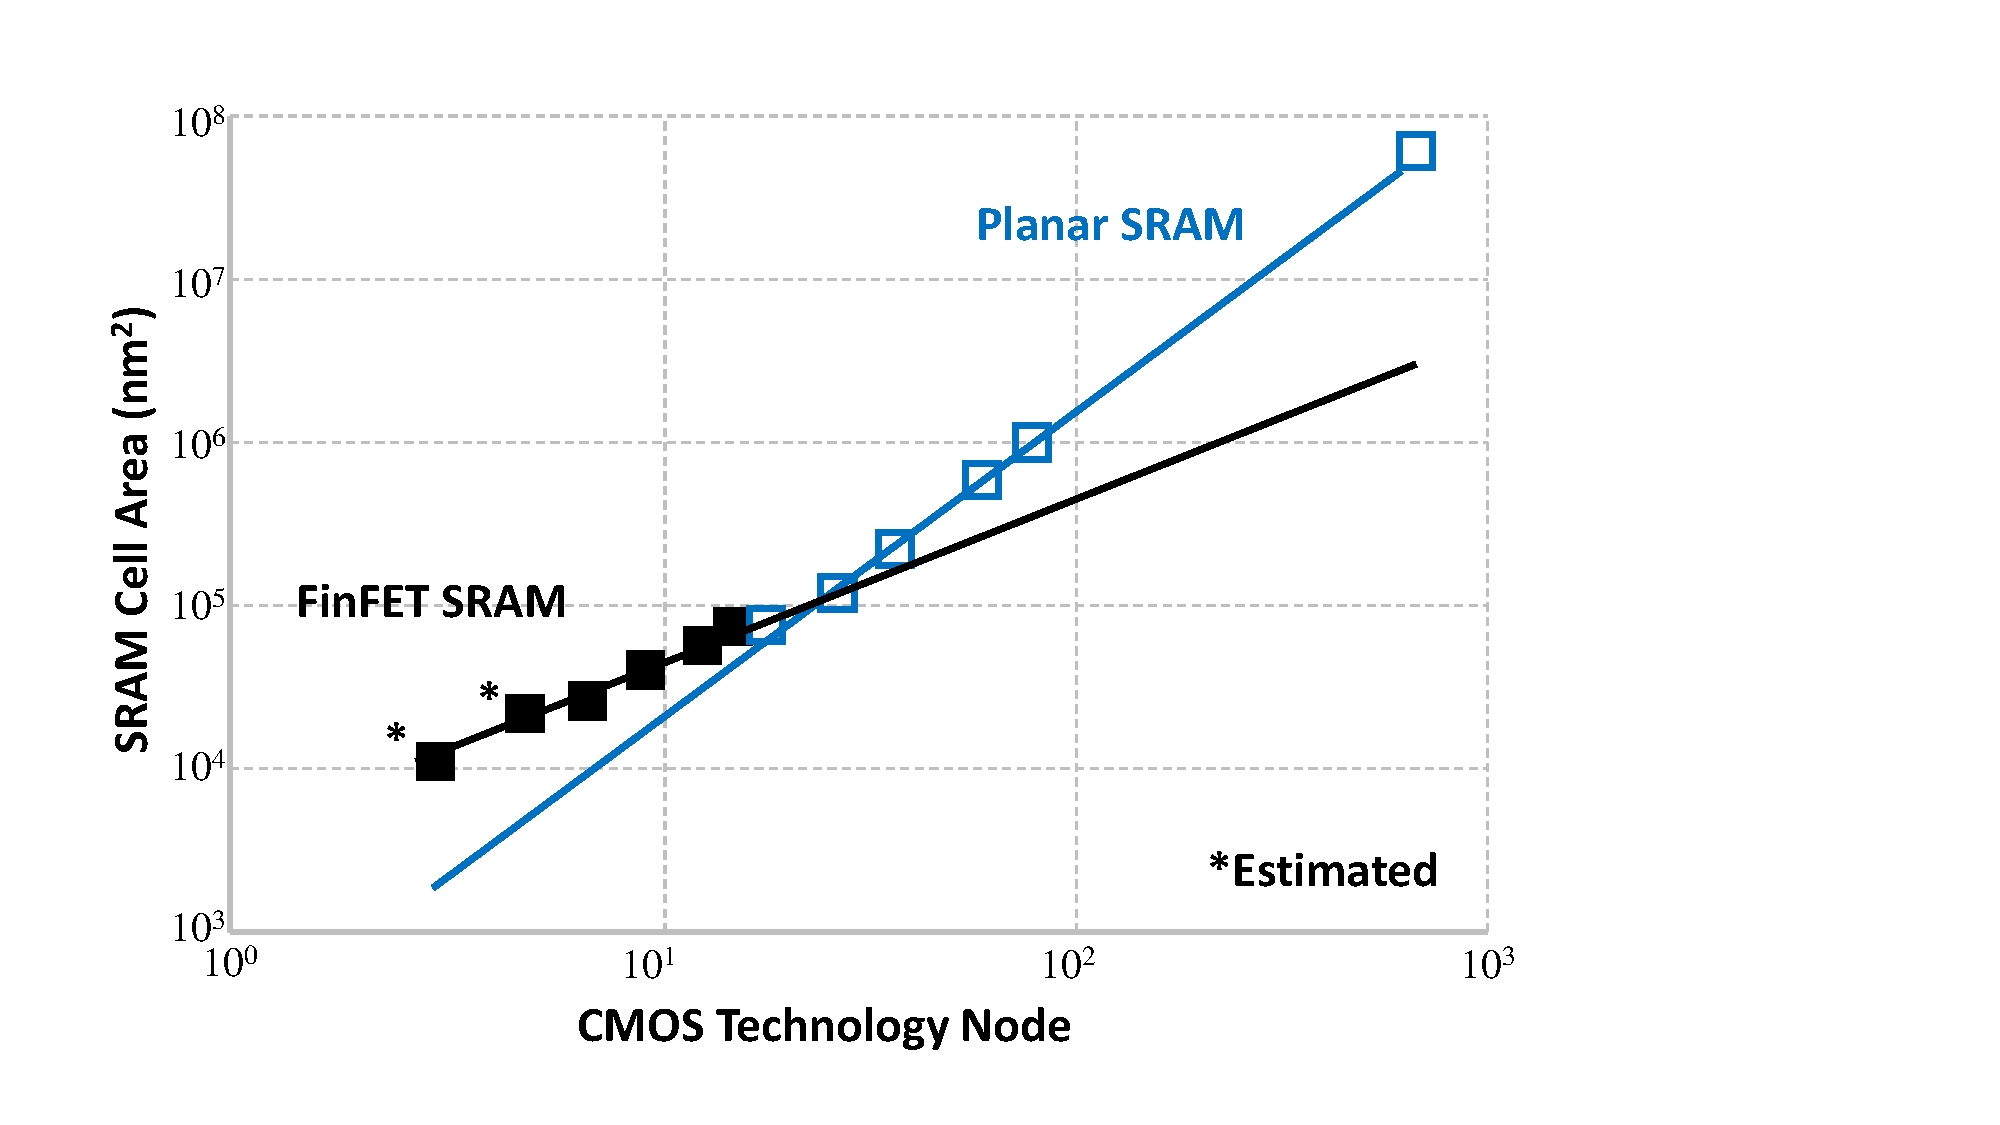
\includegraphics[width=0.7\linewidth]{example_plot}
        \caption{Here is an example figure. Make sure the caption is descriptive.}
        \label{fig:myfigure}
    \end{figure}

    \figref{fig:HTS-AT_VS_BLSTM} is an example of a complex figure with sub-figures, using the \texttt{subfig} package and \texttt{\textbackslash subfloat} commands.

    \begin{figure}[h]
        \centering
        \subfloat[\centering IEMOCAP]{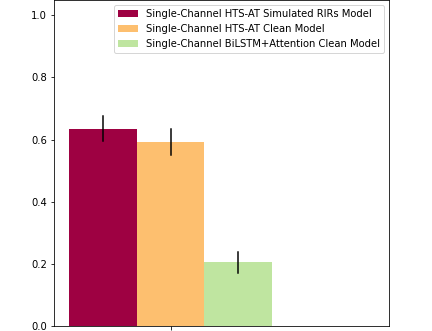
\includegraphics[width=0.53\columnwidth]
            {Figures/ACE_mp2_Lecture_Room_2_T60=1220ms_htsat_vs_blstm_IEMOCAP.png} }
        \subfloat[\centering RAVDESS]{{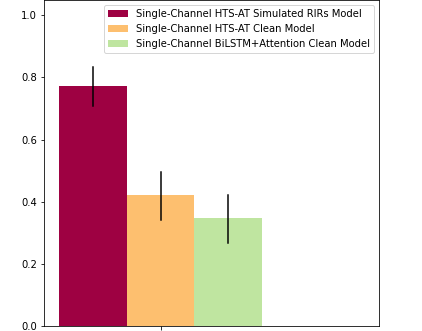
\includegraphics[width=0.52\columnwidth]
            {Figures/ACE_mp2_Lecture_Room_2_T60=1220ms_htsat_vs_blstm_RAVDESS.png} }}
        \centering
        \caption{Accuracy and Confidence Interval on test sets convolved with ACE RIR Lecture Room 2 ($T_{60}=1220~ms$). The results of two HTS-AT fine-tuned on either clean or simulated RIRs datasets compared with trained on the clean datasets.}
        \label{fig:HTS-AT_VS_BLSTM}
    \end{figure}
    
    To learn how to make article-quality figures with PowerPoint, we recommend watching the following tutorial: 
    
    \url{https://www.youtube.com/playlist?list=PLZU5hLL_713zNceifg18xNroxzeIBdJi0}.
     
\color{black}


%----------THESIS CONTENT-------------%
%-------------------------------------%
\ifthenelse{\equal{\doctype}{msc-thesis} \or \equal{\doctype}{phd-thesis}}{
    \chapter{Thesis Content}
    \color{teal}
            From this chapter and on, you should present the content of your thesis. You will probably have several chapters of content -- for example, a chapter for each contribution/published paper.
    
    \color{cyan}
        Note that it is often nice to include each chapter as a separate .tex file, using the \texttt{\textbackslash include\{filename\}} option.
        You can reduce the compile time of your paper by adding \texttt{\textbackslash includeonly\{filename\}} in the options. 
        This will only output the content of the selected file, but will retain the full file's numbering and everything.
    \color{black}
    
    \chapter{Thesis Content -- \textit{e.g., another contribution}}
    \color{teal}
        This could be a chapter about another contribution of your thesis.
    \color{black}
    
    \chapter{Thesis Content -- \textit{e.g., results}}
    \color{teal}
        This could be a chapter about the results.
    \color{black}
}


%-------RESEARCH OBJECTIVES-----------%
%-------------------------------------%
\ifthenelse{\equal{\doctype}{msc-proposal} \or \equal{\doctype}{phd-proposal}}{
    \chapter{Proposed Research}
    \section{Research Objectives}
        \label{sec_objectives}
        \color{teal}
            The main research objective of this work is to ...
        \color{black}

    \section{Proposed Research}
        \label{sec_proposed_research}
        \color{teal}
            This research constitutes the following ...
        \color{black}
        
    \section{Research Methodology}
        \label{sec_methodology}
        \color{teal}
            The methodology for carrying out the research describe above is ...
            \blue{It is good advice to use a flowchart to help describe the methodology.}
        \color{black}
    \clearpage
}

\color{cyan}
    This is how to add a table. You can also create your table in Word/Excel and include the pdf instead of dealing with \LaTeX tables. Make sure to reference all you tables in the text (e.g., \tblref{tbl:ACE_results_SER}).
    % \begin{table}[h!]
    %     \centering
    %     \caption{Here is an example table. }
    %     \label{tbl:mytable}
    %     \begin{tabular}{|c|c|}
    %          \hline
    %          something & something \\
    %          \hline
    %          something & something \\
    %          \hline
    %     \end{tabular}
    % \end{table}
\begin{table}[h]
  \renewcommand*{\arraystretch}{1.1}
  \centering
    \addtolength{\belowcaptionskip}{12pt}
    \addtolength{\abovecaptionskip}{5pt}
    \caption{Results on the test sets of the RAVDESS, IEMOCAP, and CREMA-D datasets convolved with RIR of three microphones from the ACE database. The `HTS-AT' columns are fine-tuned on reverberant single-channel audio. The `Avg mel' columns depict results where mel-spectrograms were averaged across four channels during fine-tuning and tested on three channels. The `Sum PE' columns are the Patch-Embed Summation approach fine-tuned and tested on three channels.}
    \resizebox{1.00\columnwidth}{!}{
    \begin{tabular}{l ccc ccc ccc}
      \toprule
      \multirow{ 2}{*}{Room ($T_{60}$~[ms])} &  \multicolumn{3}{c}{RAVDESS} & \multicolumn{3}{c}{IEMOCAP} & \multicolumn{3}{c}{CREMA-D} \\
      \cmidrule(lr){2-4}\cmidrule(r){5-7} \cmidrule(r){8-10}
      & HTS-AT & Avg mel & Sum PE & HTS-AT & Avg mel & Sum PE & HTS-AT & Avg mel & Sum PE  \\
      \midrule
      Lecture  1 ($638$) & 77.3 (70.6-84.0) & 80.6 (74.6-86.6) & 81.3 (74.6-87.3) & 61.3 (57.1-65.2) & 67.0 (63.0-71.0) & 67.4 (63.6-71.2) & 63.2 (60.1-66.6) & 66.4 (63.2-70.1) & 67.4 (64.2-71.0)  \\
      Lecture  2  ($1220$) & 77.3 (70.6-83.3) & 78.6 (71.3-84.6) & 82.0 (76.0-88.0) & 63.4 (59.5-67.4) & 66.1 (62.4-70.0) & 68.7 (65.0-72.4) & 65.4 (62.0-68.9) & 67.3 (64.0-70.8) & 66.0 (62.5-69.3)   \\
      Lobby  ($646$) & 78.6 (72.0-84.6) & 82.0 (76.0-88.0) & 84.0 (78.0-89.3) & 61.8 (58.0-65.8) & 64.0 (60.0-67.8) & 65.1 (61.3-68.8) & 64.2 (60.9-67.8) & 66.2 (62.8-69.8) & 66.8 (63.3-70.2)  \\
      Meeting  1 ($437$) & 73.3 (66.6-80.0) & 80.6 (74.0-86.6) & 82.6 (76.6-88.0) & 62.9 (58.9-66.9) & 66.7 (62.9-70.6) & 68.7 (65.1-72.4)  & 64.4 (61.0-67.8) & 65.7 (62.5-69.3) & 65.7 (62.2-69.0)    \\
      Meeting  2 ($371$) & 82.0 (76.0-87.3) & 83.3 (76.6-89.3) & 85.3 (80.0-90.6) & 59.5 (55.7-63.6) & 66.3 (62.4-70.3) & 64.2 (60.2-68.1) & 65.6 (62.4-69.0) & 66.6 (63.4-69.8) & 66.8 (63.6-70.2)  \\
      Office 1 ($332$) & 76.0 (69.3-82.6) & 83.3 (77.3-88.6) & 80.6 (74.0-86.6) & 63.6 (59.7-67.6) & 68.3 (64.7-72.3)  & 67.2 (63.6-71.0) & 64.1 (60.1-67.6) & 68.8 (65.4-72.4) & 67.3 (64.0-71.0)         \\
      Office 2 ($390$) & 78.6 (72.6-84.6) & 81.3 (75.3-87.3) & 82.6 (76.0-88.0) & 59.5 (55.5-63.8) & 64.7 (61.0-68.8)  & 65.4 (61.5-69.6) & 62.6 (59.4-66.1) & 64.0 (60.6-67.6) & 64.1 (60.6-67.7)       \\       
      \bottomrule
       \label{tbl:ACE_results_SER}
    \end{tabular}
    }
\end{table}

    
    For a very good tutorial on how to make professional looking tables, see the following presentation:

    \url{https://people.inf.ethz.ch/markusp/teaching/guides/guide-tables.pdf}
    
\color{black}









%-------PRELIMINARY RESULTS-----------%
%-------------------------------------%
\ifthenelse{\equal{\doctype}{msc-proposal} \or \equal{\doctype}{phd-proposal}}{
    \chapter{Preliminary Results}
    \color{teal}
        Optionally, include some preliminary results here.
    \color{black}
    \clearpage
}


%----------SUMMARY--------------------%
%-------------------------------------%
\ifthenelse{\equal{\doctype}{msc-thesis} \or \equal{\doctype}{phd-thesis}}{
    \chapter{Summary and Conclusions}
    \label{sec_conclusions}
    \color{teal}
        \section{Thesis Summary}
            Here you should conclude your work and don't forget to again emphasize your achievements (e.g., publications). 
        \section{Future Work}
            Here you should discuss future steps to build on top of your work.
    \color{black}
}

%----------BIBLIOGRAPHY---------------%
%-------------------------------------%
%\chapter*{Bibliography}
\addcontentsline{toc}{chapter}{Bibliography}
\bibliographystyle{IEEEtran}
\bibliography{bibliography/this_bibliography}

%----------   Appendix  --------------%
%-------------------------------------%
\ifthenelse{\equal{\doctype}{msc-thesis} \or \equal{\doctype}{phd-thesis}}{
    \chapter*{Appendix A:\\First Appendix}
    \addcontentsline{toc}{chapter}{Appendix A: First Appendix}
    \color{teal}
        OPTIONAL: If you require an appendix (e.g., for attaching a paper or attaching a piece of code) you can add it here.
    \color{black}
}


%------HEBREW ABSTRACT---------%
%------------------------------%
\ifthenelse{\equal{\doctype}{msc-thesis} \or \equal{\doctype}{phd-thesis}}{
    % Create your Hebrew abstract with the .docx files 
    %    under AuxiliaryPages and save as pdf. 
    \backmatter
    \pagestyle{empty}
    
\includepdf[fitpaper,pages=-,pagecommand={}]
                {AuxiliaryPages/abstract_hebrew_example}
    \clearpage
}

%------HEBREW FRONT PAGE-------%
%------------------------------%
    % Create your Hebrew front page with the .docx files 
    %    under AuxiliaryPages and save as pdf. 
    % I have provided templates for both PhD and MSc theses.
    \ifthenelse{\equal{\doctype}{msc-thesis}}{
        
\includepdf[fitpaper,pages=-,pagecommand={}] {AuxiliaryPages/front_page_hebrew_msc_thesis_example}
    }
    
    \ifthenelse{\equal{\doctype}{phd-thesis}}{
        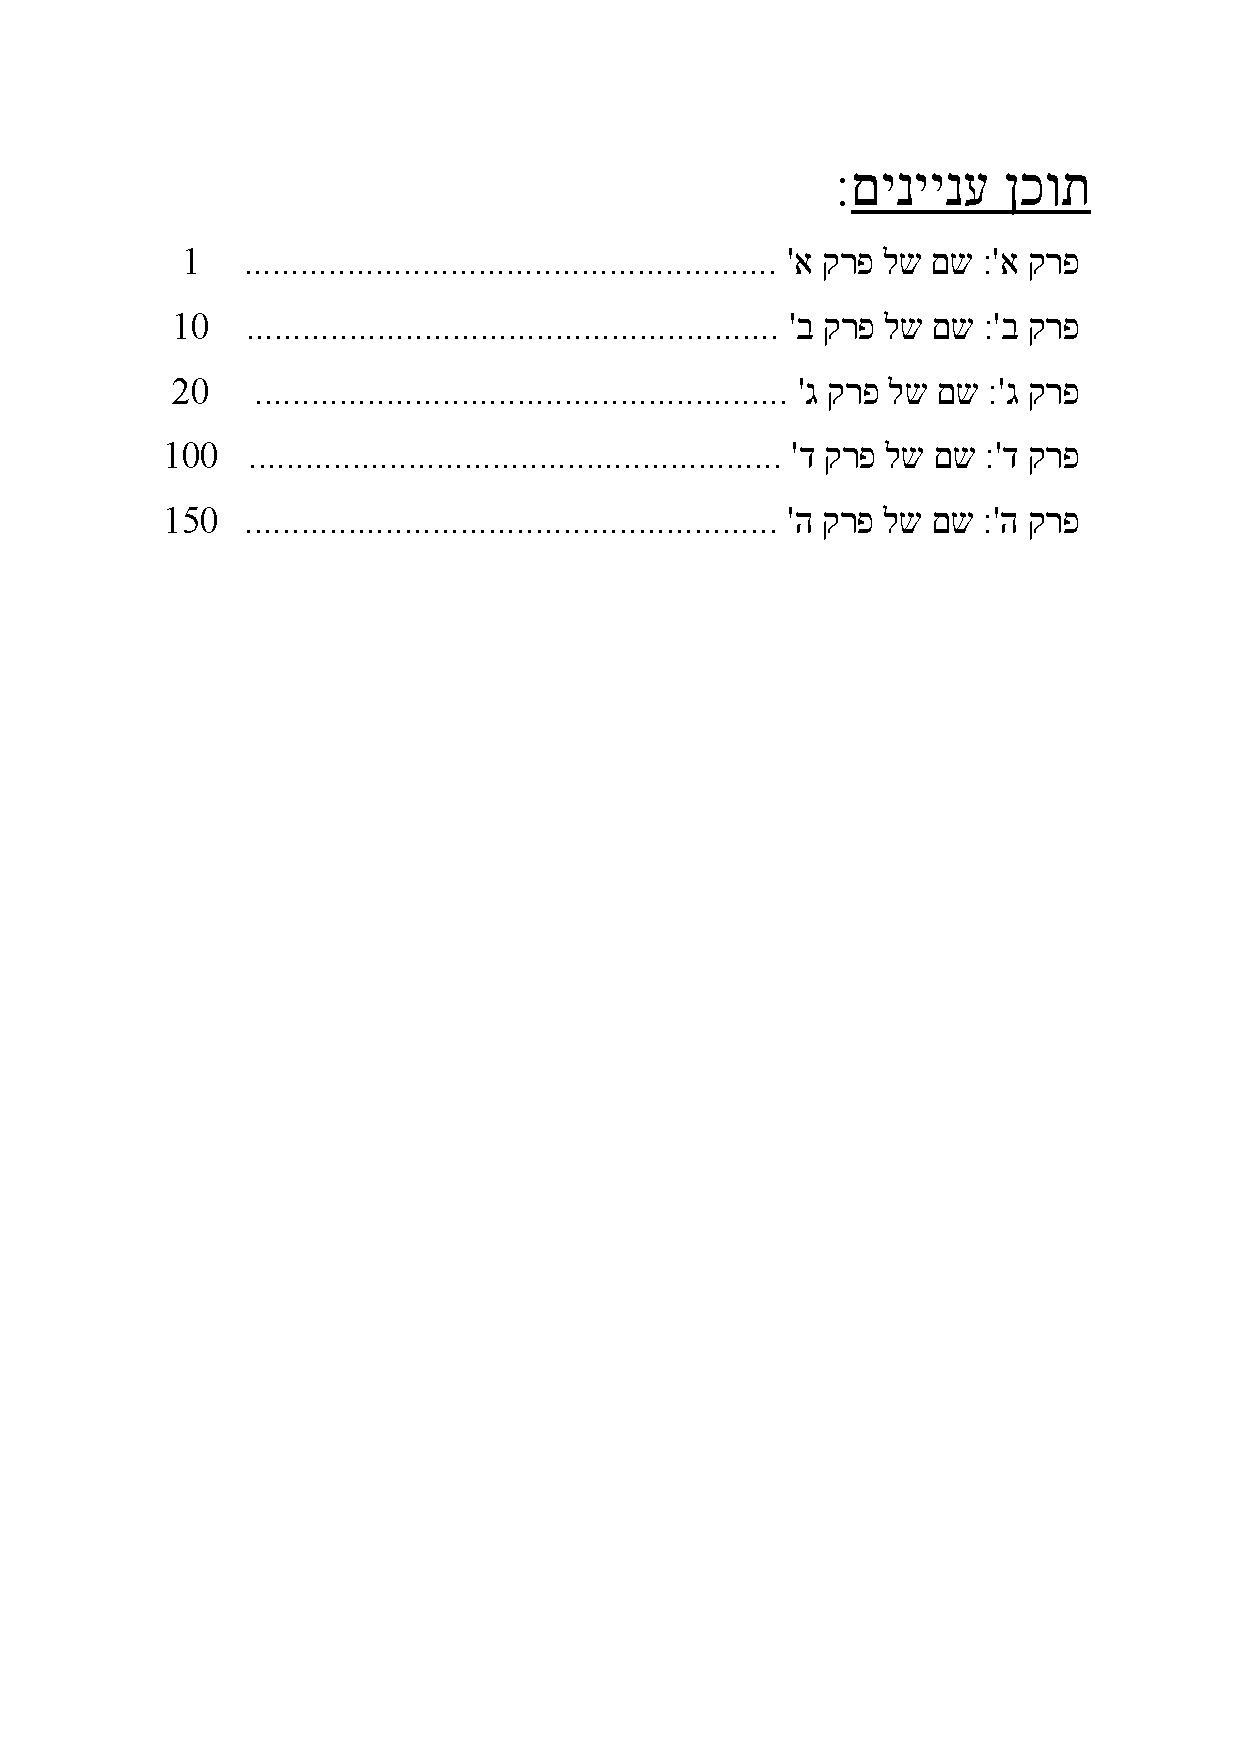
\includepdf[fitpaper,pages=-,pagecommand={}] {AuxiliaryPages/front_page_hebrew_phd_thesis_example}
    }
    \clearpage


\end{document}